\documentclass[a4paper, 12pt]{article}%тип документа

%отступы
\usepackage[left=2cm,right=2cm,top=2cm,bottom=3cm,bindingoffset=0cm]{geometry}

%Русский язык
\usepackage[T2A]{fontenc} %кодировка
\usepackage[utf8]{inputenc} %кодировка исходного кода
\usepackage[english,russian]{babel} %локализация и переносы

%Вставка картинок
\usepackage{wrapfig}
\usepackage{graphicx}
\graphicspath{{pictures/}}
\DeclareGraphicsExtensions{.pdf,.png,.jpg}

%оглавление
\usepackage{titlesec}
\titlespacing{\chapter}{0pt}{-30pt}{12pt}
\titlespacing{\section}{\parindent}{5mm}{5mm}
\titlespacing{\subsection}{\parindent}{5mm}{5mm}
\usepackage{setspace}

%Графики
\usepackage{multirow}
\usepackage{pgfplots}
\pgfplotsset{compat=1.9}

%Математика
\usepackage{amsmath, amsfonts, amssymb, amsthm, mathtools}

%Заголовок
\author{Сорокин Вадим\\
828 группа}
\title{\textbf{Работа 4.1\\
Исследование поляризации света с помощью 3D-очков}}
\newtheorem{task}{Задача}
\begin{document}
\maketitle
\section*{Цель работы}
Исследовать поляризацию света, доказать закон Малюса, проверить утверждение о том, что под углом Брюстера свет полностью поляризуется.
\section*{Оборудование}
Две пары 3D очков с технологией RealD 3D, зеркало, гладкий стеклянный предмет, матовый предмет, поверхность воды, целлофановая пленка, телефон, LCD-экран, транспортир.
\section*{Теория}
\subsection*{Плоская волна}
Из курса электромагнетизма известно, что решение уравнений Максвелла для
бегущей плоской электромагнитной волны в вакууме (и в любой другой линейной
изотропной среде) можно разложить на сумму двух решений с перпендикулярной друг другу линейной поляризацией электромагнитных волн, в каждой из которых
напряжённости электрического и магнитного полей $E$ и $H$ и направление распространения волны S представляют собой правую тройку векторов. Направлением поляризации линейно поляризованного света принято считать направление колебаний вектора E, плоскостью поляризации называют плоскость $(E, S)$.
Поля монохроматической волны, направленные вдоль осей $x$ и $y$ имеют вид
\[E_x(t) =E_{0x} \cos(\omega t + \varphi_1)\]
\[E_y(t) =E_{0y} \cos(\omega t + \varphi_2)\]
В зависимости от разницы фаз и соотношения между поляризация может быть круговой, эллиптической или плоской. Приведем примеры поляризации, когда $E_{0x} = E_{0y}$, в зависимости от $\Delta \varphi = \varphi_2 - \varphi_1$.

\begin{figure}[h]
\begin{center}
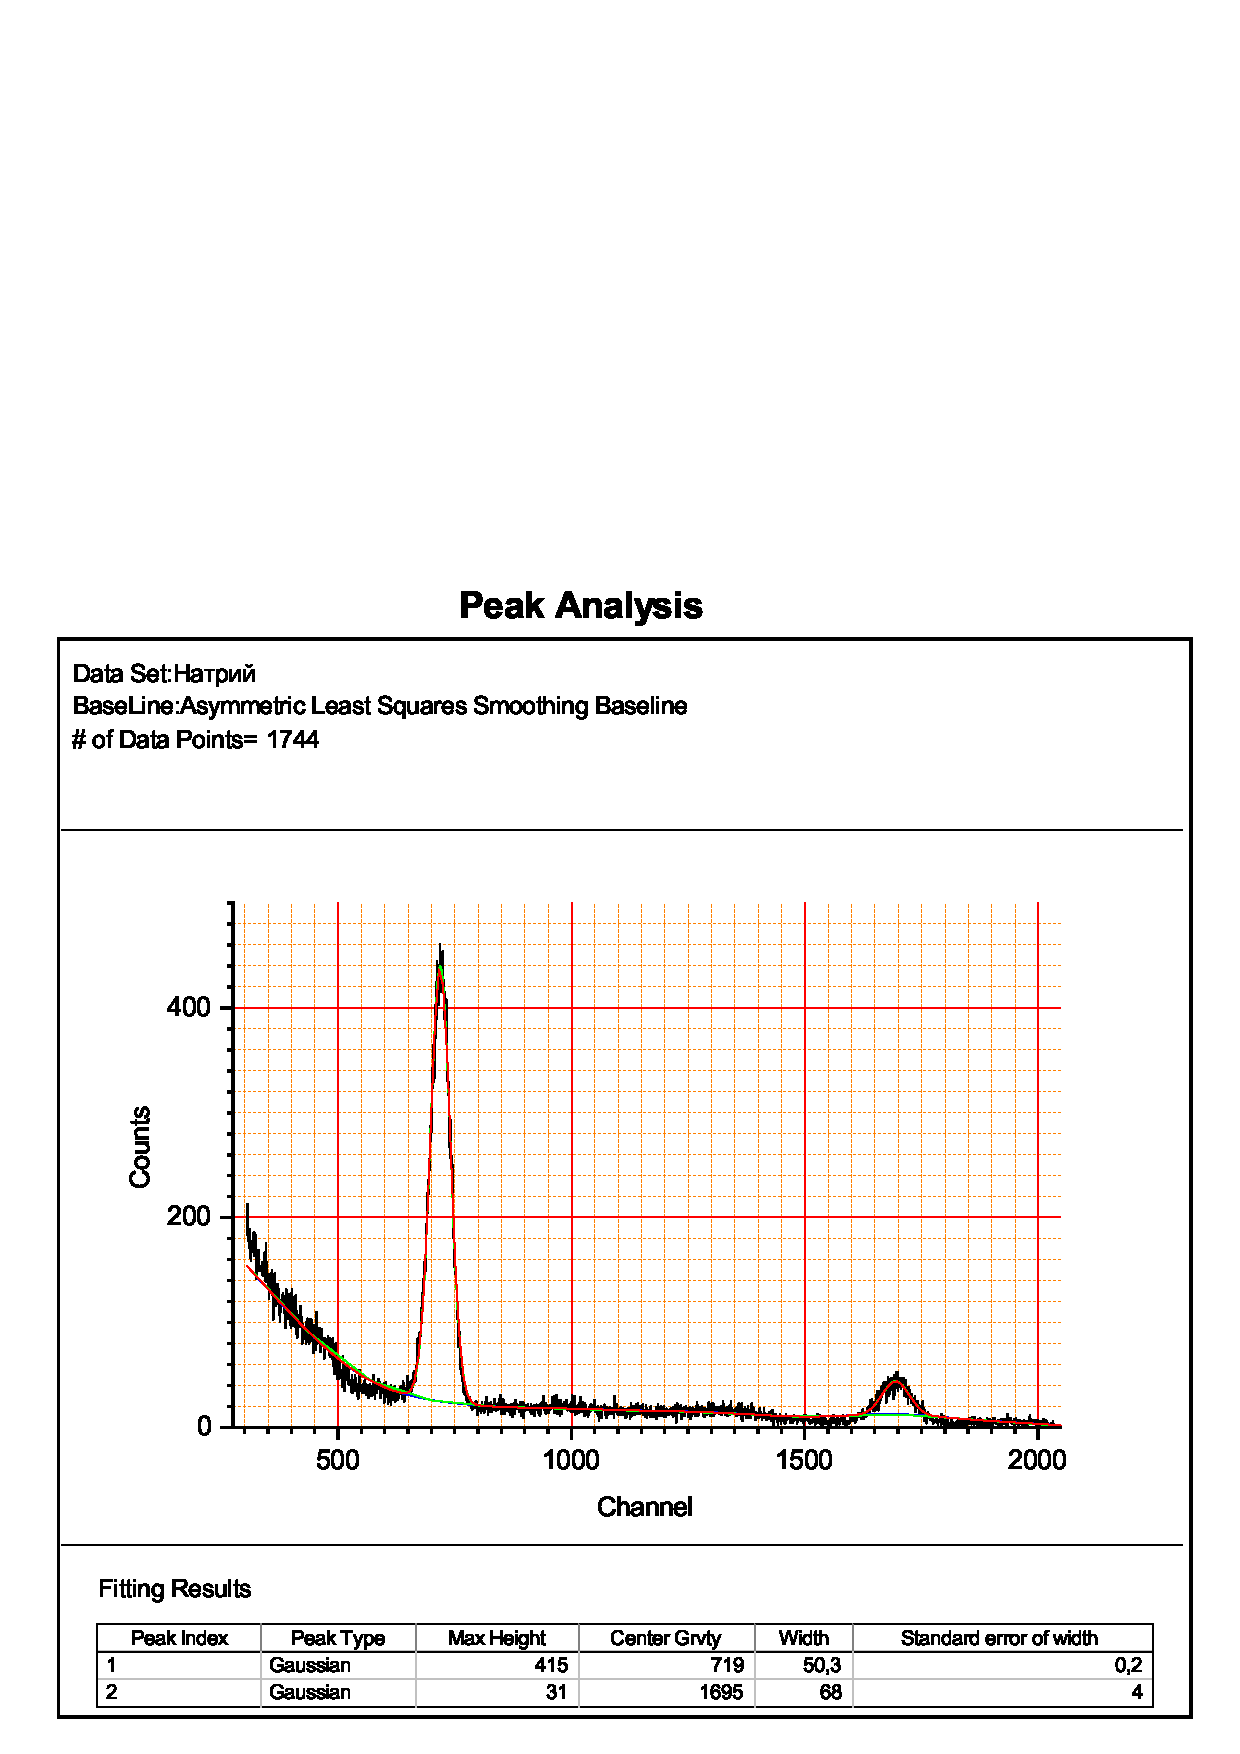
\includegraphics[width = 0.8\textwidth]{1.png}
\caption{Эллипсы поляризации в зависимости от $\Delta \varphi$}
\end{center}
\end{figure}

Весьма полезным для описания оптических систем оказывается математический
факт, что любой эллиптически поляризованный свет можно представить как суперпозицию лево- и право циркулярно поляризованного света (круговая поляризация), либо на сумму линейных поляризаций по любым непараллельным друг другу осям. Доказательство этого факта представляется читателю в качестве упражнения, можно только отметить что эллиптически поляризованный свет представляется как сумма двух линейных компонент вдоль главных осей эллипса с разницей фаз $\pi/2$, каждая же из линейных компонент может быть представлена как суперпозиция двух круговых поляризаций, либо как сумма линейных поляризаций по любым двум осям.
\subsection*{Закон Малюса}
Он является весьма очевидным, если мы вспомним разложение любой эллиптической (в том числе вырожденный эллипс) волны на 2 круговые по перпендикулярным составляющим. Тогда
\[E_1 = E_0 \cos \varphi\]
\[E_2 = E_0 \sin \varphi\]
$\varphi$ --- угол между направлением поляризации света и разрешенным для поляроида. Эти формулы весьма очевидны, поскольку именно так гасятся волны в поляроиде. Причем, в сам поляроид пройдет только 1 компонента, поскольку вторая ему перпендикулярна, тогда
\[\frac{I}{I_0} = \frac{E_1^2}{E_0^2} = \cos^2\varphi\]
Последняя формула и представляет из себя закон Малюса.
\subsection*{Угол Брюстера}
Как известно из курса оптики, свет отражённый от гладкой поверхности приобретает частичную поляризации. Если падение из среды 1 на границу раздела сред 1 и 2 происходит под углом Брюстера 
\[\tg \theta = \frac{n_2}{n_1},\] то отражённый свет полностью линейно поляризован, при этом отражается только компонента с линейной поляризацией параллельной плоскости зеркала.
\section*{Ход работы}
\begin{enumerate}
\item Наденем очки и посмотримся в зеркало, закрывая левый и правый глаз мы видим, что у нас не затемнена та линза, за которой закрытый глаз, когда если открыты оба глаза, то затемнены оба глаза. Если же мы повернем очки дужками наружу, то мы всегда видим, что глаза не затемнены. Это значит, что очки состоят из поляризационного фильтра и пластинка $\lambda/4$. Почему? 

Потому что в если мы смотрим одним глазом когда очки не развернуты, то луч с естественной поляризацией проходит через поляризатор, после чего он приобретает линейную поляризацию, которую пластинка превращает в круговую, затем поскольку пластинки подобраны так, что при прохождение через одну, у нас получается левая поляризация, а через другую --- правая, то тогда, при прохождении через ту же пластину, она приобретет перпендикулярную поляризацию, по сравнению с фильтром, который располагается под ним, именно поэтому мы не видим глаз которым смотрим, а если пройдет через другую, то поляризация будет сонаправлена фильтру, поэтому мы видим другой глаз, а мы видим все, если развернуть очки, потому что у самих поляризаторов направление поляризации согласовано.

\item Экран гасится, поскольку мы просто делаем систему такой, что свет проходит сразу 2 поляризатора, и при вращении, если добиться того, что у поляризаторов перпендикулярны разрешенные направления, то мы получим гашение света.

При сложении внешними частями, у нас свет сначала поляризуется линейно, потому из него превращается в свет с круговой поляризацией, затем он опять становится линейным, а там он гасится или не гасится в зависимости от совпадения или несовпадения линейной поляризации пластины и разрешающего направления фильтра. Возможная причина, из-за чего у нас изменяется цвет, это явление дисперсии, из-за чего у каждого цвета при линейной поляризации есть свое небольшое отклонение от среднего угла плоской поляризации, а из-за того, что мы взяли разные очки, у которых пластины и фильтры не подстроены друг под друга, фильтр из второй пары очков пропускает часть света определенного цвета, этот вывод можно сделать из того, что мы всегда видим оттенки либо красного, либо синего.
\item Проверим закон Малюса, для этого соберем установку: возьмем рамку, и сделаем на ней из ниток перпендикулярный крест, вокруг которого в дальнейшем мы будем вращать нашу линзу, приклеенную к круговому диску с нанесенными засечками под углы. На рамке сделаем засечку, по которой потом будем отсчитывать наш угол. Затем с помощью телефона, каждый раз фокусируясь на одно и то же место сделаем ряд фотографий для каждого угла, который смотрим. Затем возьмем квадрат 10 на 10 пикселей в самой темной части линзы и будем следить за его яркостью. Затем в мной написанной программе в системе ARGB будем следить за средним яркости этого квадрата. Среднее с погрешностью будем заносить в таблицу, среднее погрешности считаем как среднее квадратичное, а именно 
\[\delta x = \frac{1}{\sqrt{100\cdot99}}\sqrt{\sum\limits_{i = 1}^{100} \left(x_i - \overline{x}\right)^2}\]
Затем, взяв за погрешность угла $\delta \varphi = 2,5^{\circ}$, рассчитаем погрешность для $\cos^2\varphi$
\[\delta\left( \cos^2\varphi\right) = \cos^2\varphi \cdot \left| \dfrac{\partial \cos^2 \varphi}{\partial\varphi}\right| \varepsilon_{\varphi} = 2 \cos^3\varphi \cdot \sin\varphi \cdot \varepsilon_{\varphi}\]
Затем, предположив, что интенсивность пропорциональная яркости, построим график зависимости яркости от $\cos^2\varphi$.

Перед всеми измерениями устанавливаем так называемый ноль: когда поляризации перпендикулярны, то есть когда за линзой ничего не видно, и уже относительно него, считая что если поляризации перпендикулярны, то это $90^{\circ}$ считаем $\varphi$
\begin{table}[h]
\begin{center}
\begin{tabular}{|c|c|c|c|c|}
\hline
$\varphi$ & Яркость, у.е. & $\cos^2\varphi$ & $\delta(\cos^2\varphi)$ & $\delta$ Яркость \\ \hline
90        & 450           & 0               & 0,01                    & 200              \\ \hline
85        & 550           & 0,01            & 0,01                    & 200              \\ \hline
80        & 600           & 0,03            & 0,01                    & 200              \\ \hline
75        & 700           & 0,07            & 0,01                    & 200              \\ \hline
70        & 750           & 0,12            & 0,01                    & 200              \\ \hline
65        & 900           & 0,18            & 0,01                    & 200              \\ \hline
60        & 1100          & 0,25            & 0,02                    & 200              \\ \hline
55        & 1600          & 0,33            & 0,02                    & 200              \\ \hline
50        & 1800          & 0,42            & 0,03                    & 200              \\ \hline
45        & 2100          & 0,5             & 0,1                     & 200              \\ \hline
40        & 2400          & 0,6             & 0,1                     & 200              \\ \hline
35        & 2500          & 0,7             & 0,1                     & 200              \\ \hline
30        & 2600          & 0,8             & 0,1                     & 200              \\ \hline
25        & 3000          & 0,8             & 0,1                     & 200              \\ \hline
20        & 3200          & 0,9             & 0,1                     & 200              \\ \hline
15        & 3400          & 0,9             & 0,2                     & 200              \\ \hline
10        & 3400          & 1               & 0,2                     & 200              \\ \hline
5         & 3500          & 1               & 0,2                     & 200              \\ \hline
0         & 3500          & 1               & 0,2                     & 200              \\ \hline
\end{tabular}
\caption{Зависимость яркости от угла, с погрешностями}
\end{center}
\end{table}

\begin{figure}[h]
\begin{center}
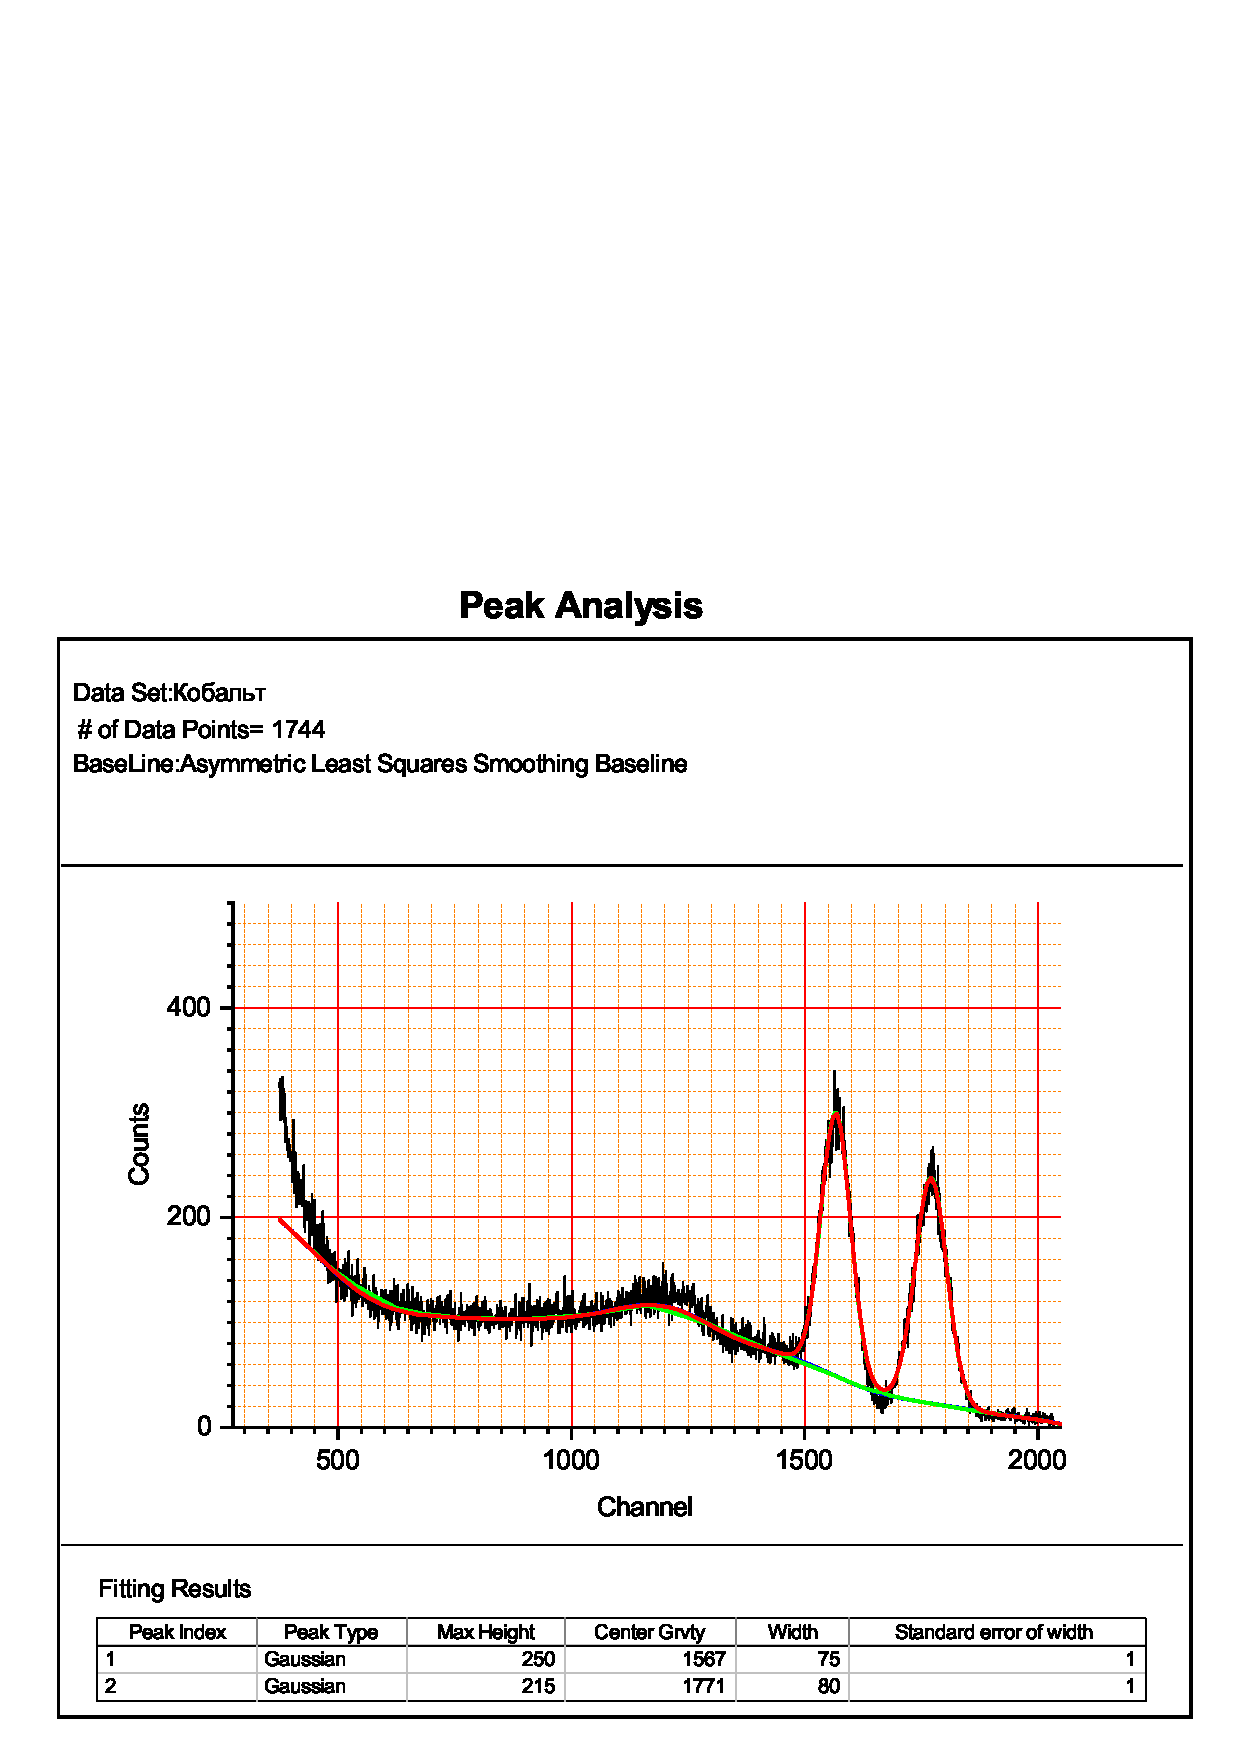
\includegraphics[width = 0.2\textwidth]{2.jpg}
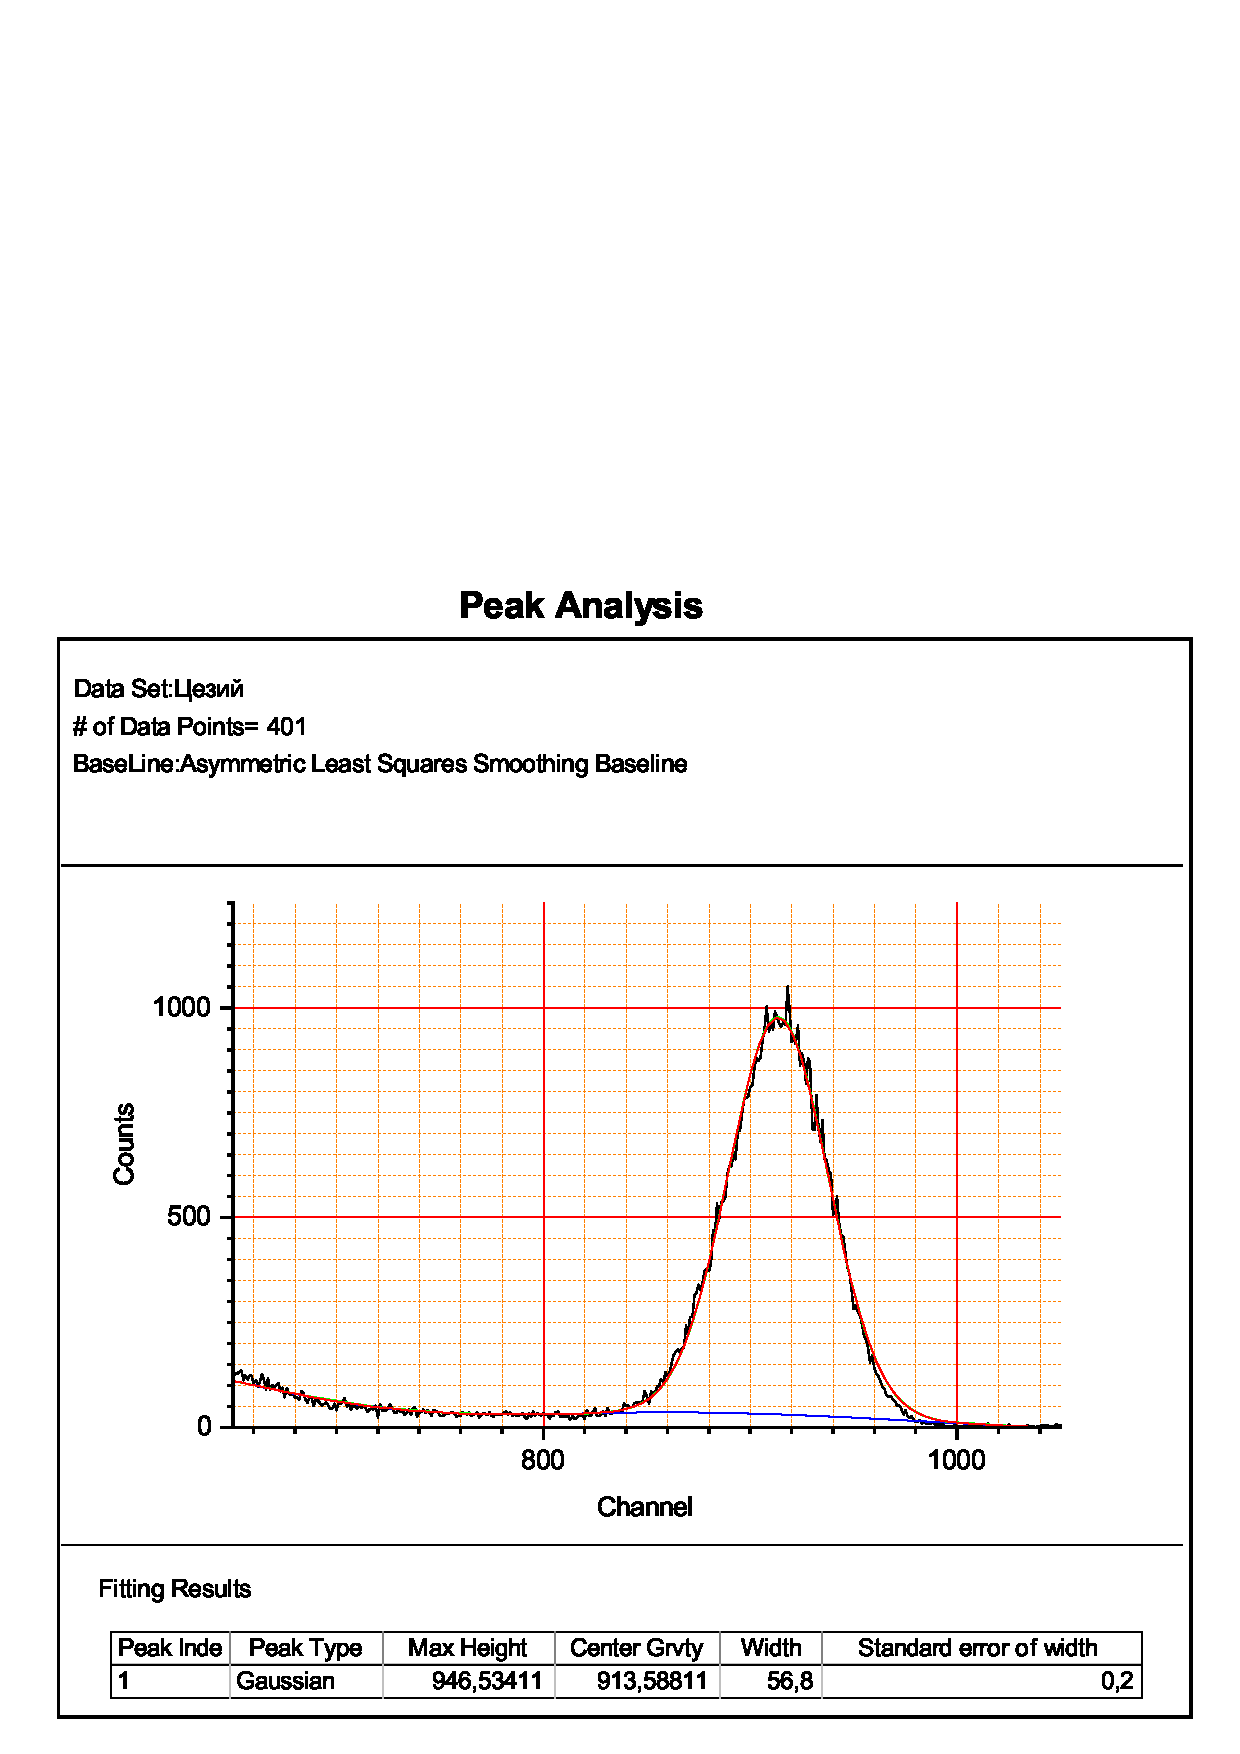
\includegraphics[width = 0.2\textwidth]{3.jpg}
\includegraphics[width = 0.2\textwidth]{4.jpg}
\caption{Некоторые примеры фотографий, по которым выявлялась зависимость}

\end{center}
\end{figure}

\begin{figure}[h]
\begin{center}
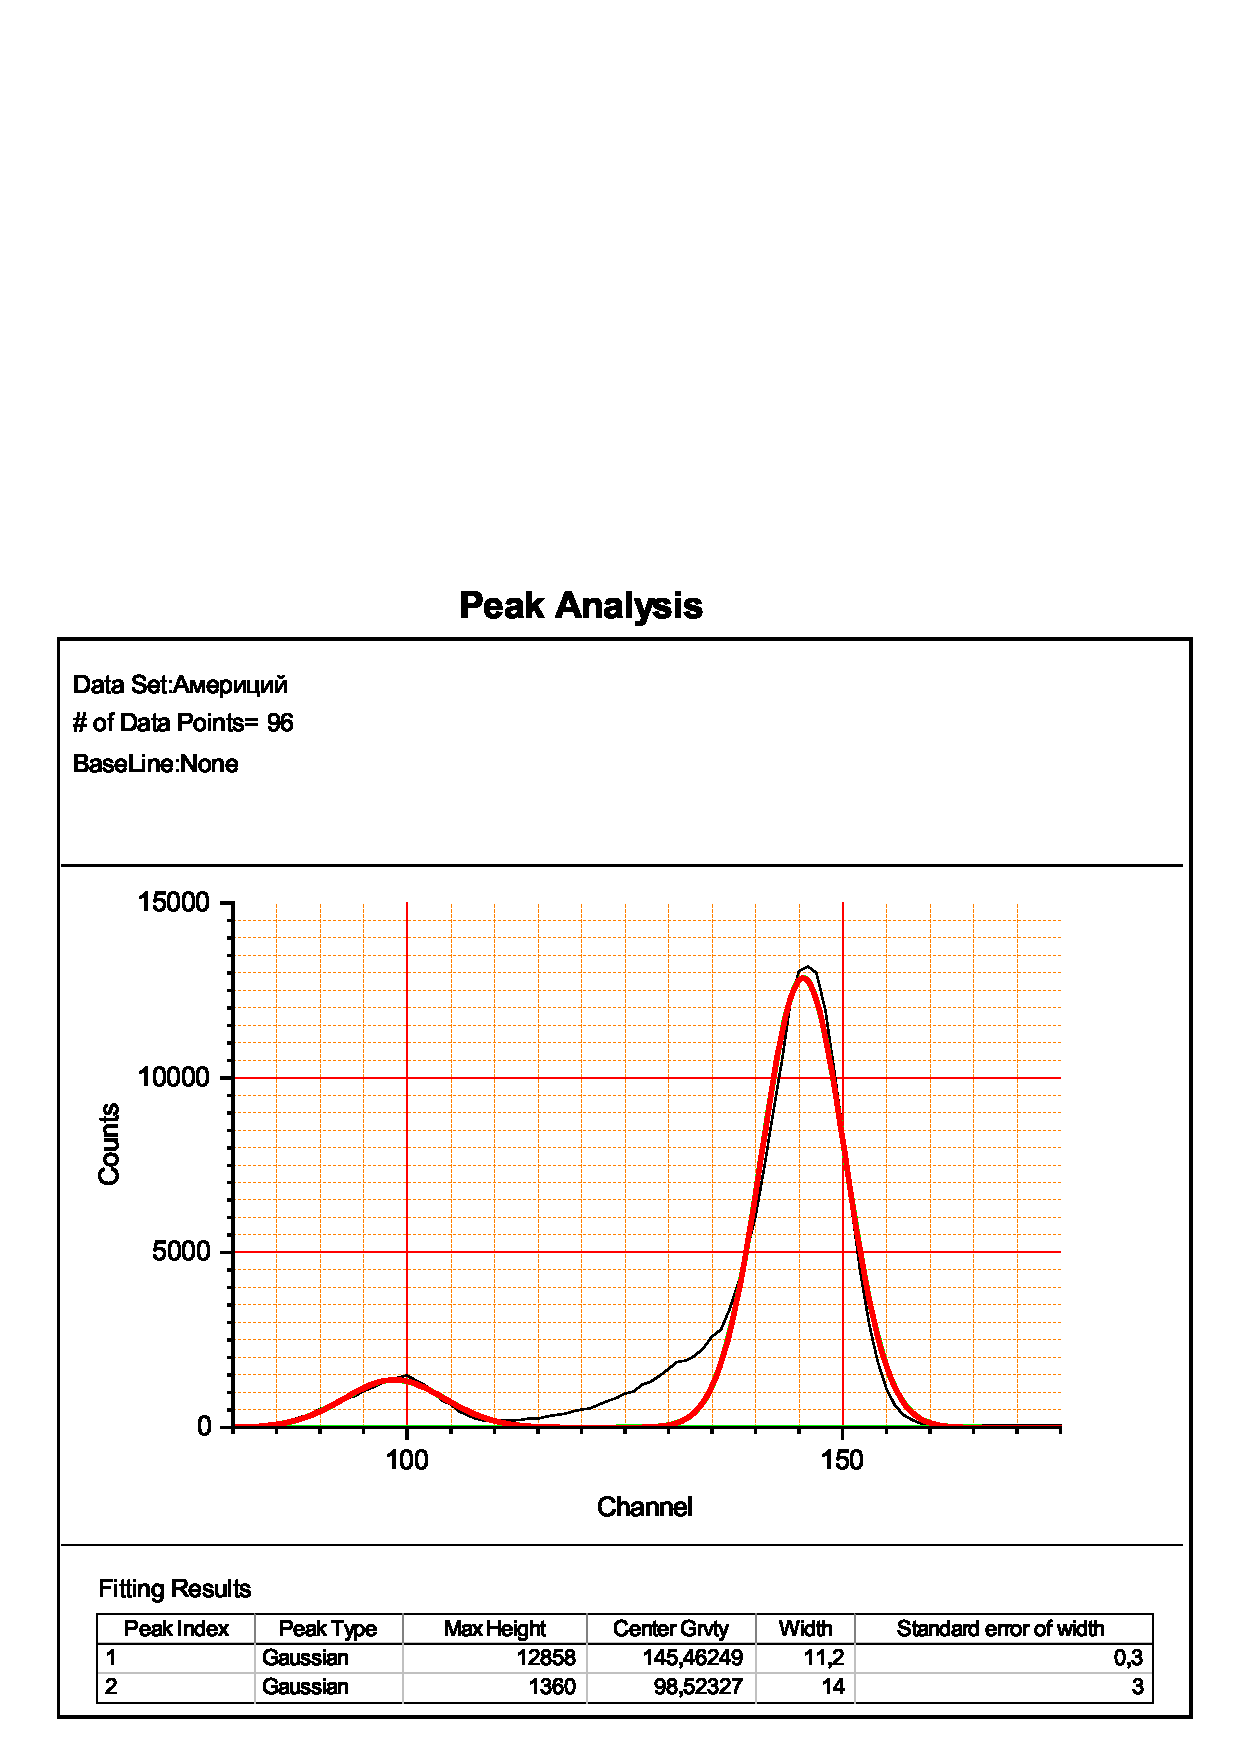
\includegraphics[width = 0.7\textwidth]{5.jpg}
\caption{График зависимости яркости от квадрата косинуса угла}
\end{center}
\end{figure}
\item Определим по углу Брюстера, из соображений, высказанных в теории, что у одной линзы поляризация вертикальная, у другой горизонтальная, так как при наблюдении под углом Брюстера, мы должны очки повернуть на 90$^{\circ}$, чтобы лампа исчезла, для одной линзы, и не надо поворачивать для другой. Собрав установку, а именно двигающийся блок относительно блюда с водой мы определяем $\tg \theta = a/b$, где $a$ --- высота, на которой стоит линза, относительно поверхности, а $b$ --- расстояние до пятна (подберем так, чтобы было на краю блюда). Аналогично сделаем со стеклом, только в этот раз мы будем измерять непосредственно угол, так как у нас будет неподвижны фильтр и лампа, но вертеться стекло $\Rightarrow$. Для воды получаем $a = (23 \pm 1) cm, b = (18\pm 1)cm \Rightarrow n_{water} = \tg\theta = 1,3 \pm 0,1$, что почти совпадает с реальным значением $1,33$, несмотря на неточность эксперимента. Аналогично проделываем со стеклом, $\theta = (60\pm 2,5)^{\circ}  \Rightarrow n_{steklo} = 1,7 \pm 0,1$. Для стекла находим погрешность аналогично $\cos^2\varphi$.
\item Попробовал внести между очками целлофан, интересных эффектов, отличающихся от предыдущих не обнаружил.
\end{enumerate}
\subsection*{Вывод}
Мы изучили эффект поляризации света, проверили справедливость, с некоторой точностью Закона Малюса, и убедились в свойствах Угла Брюстера.
\subsection*{Литература}
\begin{enumerate}
\item Сивухин Д. В. Оптика//Общий курс физики //М.: Физматлит. – 2006. – Т. 4. – 792 С.
\item Практикум по физической химии / под ред. С.В. Горбачева// – М.: Высшая школа,
1974. – 496 С. (С. 354)
\end{enumerate}
\end{document}
